%+----------------------------------------------------------------------------+
%| SLIDES: 
%| Chapter: Brief introduction to multisymplectic geometry and Homotopy momap
%| Author: Antonio miti
%| Event: PHD preliminary Defence
%+----------------------------------------------------------------------------+

%- HandOut Flag -----------------------------------------------------------------------------------------
\newif\ifHandout

%- D0cum3nt ----------------------------------------------------------------------------------------------
\documentclass[beamer,handout,10pt]{standalone}
	\setbeameroption{show notes}
	



%- Packages ----------------------------------------------------------------------------------------------
%\usepackage{verbatim}
\usepackage[mode=buildnew,subpreambles=true]{standalone}
\usepackage{import}
\usepackage{amsmath, amssymb}
\usepackage{tikz}
%\usetikzlibrary{arrows,shapes,calc}
%\usetikzlibrary{shapes.callouts}
\usepackage{tikz-cd}
\usepackage{hyperref}
\usepackage[english]{babel}
\usepackage{stackengine}

%--Beamer Style-----------------------------------------------------------------------------------------------
\usetheme{toninus}



%--Beamer Style-----------------------------------------------------------------------------------------------
\usetheme{toninus}



%-----------------------------------------------------------
% Define a whole bunch of custom colours and fonts
%-----------------------------------------------------------
\definecolor{lgreen} {RGB}{180,210,100}
\definecolor{dblue}  {RGB}{20,66,129}
\definecolor{ddblue} {RGB}{11,36,69}
\definecolor{lred}   {RGB}{220,0,0}
\definecolor{nred}   {RGB}{224,0,0}
\definecolor{norange}{RGB}{230,120,20}
\definecolor{nyellow}{RGB}{255,221,0}
\definecolor{ngreen} {RGB}{98,158,31}
\definecolor{dgreen} {RGB}{78,138,21}
\definecolor{nblue}  {RGB}{28,130,185}
\definecolor{jblue}  {RGB}{20,50,100}
\definecolor{lincolngreen}{rgb}{0.11, 0.35, 0.02}



\usepackage{lmodern}
\usepackage{empheq}
\renewcommand{\d}{\ensuremath{\operatorname{d}}}

%---------------------------------------------------------------------------------------------------------------------------------------------------
%- D0cum3nt ----------------------------------------------------------------------------------------------------------------------------------
\begin{document}
%------------------------------------------------------------------------------------------------



%----------------------------------------------------------------------------------------------------------------------------------
\begin{frame}{Goal}
		%+---------------------------------+
		%| Goals                           |
		%+---------------------------------+
		\begin{block}{Introduction and Goals}
			\vspace{0.5em}
			\centering
			\parbox{0.98\linewidth}{%
			\emph{
				{\color{lincolngreen!80!black} Multisymplectic manifolds}, 	
				{\color{norange!80!black}$L_\infty$ observables} and 
				{\color{nred!80!black}homotopy co-moment maps} are 
				\underline{higher generalizations} of (resp.)
				{\color{lincolngreen!80!black} symplectic manifolds}, 
				{\color{norange!80!black} Poisson algebras} and 
				{\color{nred!80!black}co-moment maps}. %ectively.
				\\
				Being the latter a particularly subtle and technical concept, 
				we worked out some new meaningful concrete examples of possible interests in different fields of mathematics.
			}
			}
			\vspace{.5em}
		\end{block}
\end{frame}
%----------------------------------------------------------------------------------------------------------------------------------



%----------------------------------------------------------------------------------------------------------------------------------
\begin{frame}[shrink]
	%+------------------------------+
	%| L Structures									 |
	%+------------------------------+
	\begin{block}{$L_\infty$ Algebras}
		\vspace{.5em}
		\centering
		\parbox{0.98\linewidth}{%
		\emph{
			$L_\infty$-algebra is the notion that one obtains from a Lie algebra when one requires the Jacobi identity to be satisfied only up to a higher coherent chain homotopy.
		}
		}
		\\
		\vspace{.5em}
		\begin{defblock}[$L_\infty$-algebra \emph{(Lada, Stasheff)}]
			\includestandalone{Pictures/Figure_Linfinitydef}
		\end{defblock}	
		%
		%
		\begin{columns}[c]
			\hfill
			\begin{column}{0.5\linewidth}
				Higher Jacobi implies:
				\begin{itemize}
					\item Underlying chain-complex $(L,\mu_1)$;
					\item \color{nred} $\mu_2$ is a chain map $L^{\otimes 2} \to L$;
					\item \color{lincolngreen}$\mu_3$ is a chain homotopy 
						$\mu_2\circ\mu_2 \Rightarrow 0$;
					\item \color{purple}higher analogues...	
				\end{itemize}
			\end{column}
			\begin{column}{0.45\linewidth}
				\includestandalone[width=0.9\linewidth]{Pictures/Figure_Linfinity_diagram}
			\end{column}	
		\end{columns}	
		%

	\end{block}




\end{frame}
%----------------------------------------------------------------------------------------------------------------------------------



%----------------------------------------------------------------------------------------------------------------------------------
\begin{frame}
		\vspace{-.5em}
		\centering
		\parbox{0.98\linewidth}{%
		\emph{
			A powerful and unifying finite dimensional portrait suitable for the description of a rich variety of physical systems.
		Multisymplectic means \emph{"going higher"} in the degree of $\omega$.
		}
		}
		\\
		\begin{center}\begin{tabular}{p{0.2\linewidth} p{0.15\linewidth} p{0.3\linewidth}}
		Geometry: & & Mechanics: \\
		symplectic &\centering $\rightsquigarrow$ & classical point-like systems \\
		multisymplectic &\centering $\rightsquigarrow$ & classical field-like systems
		\end{tabular}\end{center}

\end{frame}
%----------------------------------------------------------------------------------------------------------------------------------



%----------------------------------------------------------------------------------------------------------------------------------
\begin{frame}[shrink]{Homotopy co-moment maps (HCMM)}	
	%+---------------------------------+
	%| Homotopy co-moment maps					|
	%+---------------------------------+

		\begin{tabular}{lll}
			\quad Consider: 
			&$\quad\bullet\quad$
			& $v:\mathfrak g\to \mathfrak X(M)$  a Lie algebra morphism 
			s.t. $\mathcal{L}_{v_x}\omega=0 \quad  \forall x\in\mathfrak g$\\
			& & \emph{(infinitesimal multisymplectic Lie algebra action $\mathfrak{g}\circlearrowleft (M,\omega)$)}
		\end{tabular} 
		%
		\vspace{.5em}
		\begin{defblock}[Homotopy co-moment maps \emph{(Callies, Fregier, Rogers, Zambon)}]
			\vspace{.25em}
			\centering
			\parbox{0.96\linewidth}{%
  				$L_\infty$-morphism $\quad(f): \mathfrak{g} \to L_\infty(M,\omega)$
  				 \quad such that \quad
  				 $d f_1 (\xi) = -\iota(v_\xi) \omega $ $\forall \xi \in \mathfrak{g}$.
  		}
		\end{defblock}
		%
		\begin{columns}
			%
			\begin{column}{.625\textwidth}			
				\begin{propblock}[HCMM unfolded]
					%
					\begin{displaymath}
						(f)  = \big\{ f_i: \,\,\, \Lambda^i {\mathfrak g} \to \Omega^{n-i}(M)
						\quad \vert \quad 
						0\leq i \leq n+1  \big\}	
					\end{displaymath}
					%
					\begin{displaymath}
						\begin{split}
							\text{fulfilling:}\quad
							\bullet\quad & f_0 = f_{n+1} = 0
							\\
							\bullet\quad & d f_k (p) = f_{k-1} (\partial p)  
							+ \varsigma(k) \iota(v_p) \omega
							\; ~( := \mu_k )
						\end{split}
					\end{displaymath}	
					for all $p \in \Lambda^k\mathfrak{g}$ and $k=1,\dots n+1$.	
					\footnotetext{Notation: \qquad $\partial =$ Chevalley-Eilenberg boundary operator.}
				\end{propblock}
			\end{column}
			%
			\begin{column}{.375\textwidth}
				%
				\begin{propblock}[Conservation\\ of momenta]
					Fixed $H\in \Omega^{n-1}_{\text{Ham}}(M)$, $\mathfrak{g}$-invariant,
					\begin{displaymath}
					\begin{split}
						\mathcal{L}_{v_H} f_k(p) \in B^k&(M) \\
						& \forall p \in Z_k(\mathfrak{g}) ~.
					\end{split}
					\end{displaymath}
					\footnotetext{
						\begin{tabular}{c c}
							Notation: &\qquad $B^k(M) =$ exact $k$-forms,\\
							&\qquad $Z_k(\mathfrak{g}) =$ C.-E. cycles.
						\end{tabular}
					}
				\end{propblock}
			\end{column}
		\end{columns}

\end{frame}
%----------------------------------------------------------------------------------------------------------------------------------



%----------------------------------------------------------------------------------------------------------------------------------
\begin{frame}[fragile]
	\begin{itemize}
		\item[$\blacktriangleright$] 
		$\{\text{velocity fields of incompressible fluid}\}
		\leftrightsquigarrow 
		\mathfrak{g} \subset \rm{Lie}( \rm{SDiff}(\mathbb{R}^3))$
	\end{itemize}

	\begin{propblock}[Explicit HCMM for $\rm{SDiff}_0 \circlearrowright (\mathbb{R}^3,\nu)$]
			%
		\begin{columns}[T]
			\hfill
			\begin{column}{.45\linewidth}
				\vspace{0.5em}
				\begin{empheq}[box=\fbox]{align*}
					f_1 ~=&~\flat\cdot{\rm curl}^{-1}
					\\
					f_2 ~=&~ \Delta^{-1} \delta \mu_2
				\end{empheq}
				%
				\vspace{-0.5em}
				where:
				\begin{displaymath}
					\begin{split}
						~\bullet~ \delta = \ast \cdot \d \cdot \ast 
						\qquad
						& ~\bullet~ \Delta  = \delta \cdot \d
						\\
						~\bullet~ \rm{div}   = \ast \cdot \d \cdot \alpha
						\qquad
						& ~\bullet~ \rm{curl}  = \sharp \cdot \ast \cdot \d \cdot \flat	
					\end{split}
				\end{displaymath}
				come from the standard Riemannian structure of $\mathbb{R}^3$.									
			\end{column}	
		  	\hfill  	
			\begin{column}{.5\linewidth}
				\centering
				\vspace{0.5em}
		  		\includestandalone[height=0.5\textwidth]{Pictures/Figure_Euclid_Trigger}
		 	\end{column}
		\end{columns}
	\end{propblock}
		%
	\begin{itemize}
		\item[$\blacktriangleright$]  Transgressing $(f)$ to the loop space yields the 
	 	\emph{Arnol'd-Marsden-Weinstein "hydrodynamical"} co-momentum map. 
	\end{itemize}
		 	%$(f)$ transgresses, via the evaluation map ${\rm ev}: L{\mathbb R}^3 \times {\mathbb R} \ni (\gamma, t) \mapsto \gamma(t) \in {\mathbb R}^3$ to the hydrodynamical co-momentum map of Arnol'd and Marsden-Weinstein.%
		 	 	%, defined on the Brylinski manifold $Y$ of oriented knots. \par



\end{frame}
%----------------------------------------------------------------------------------------------------------------------------------


\begin{frame}
	\begin{propblock}[Explicit HCMM for $SO(n) \circlearrowleft \left( S^{n}, \omega\right)$ for all $n \geq 2$]
		\begin{columns}[T]
			\begin{column}{.5\linewidth}
				\vspace{0.5em}
				\begin{empheq}[box=\fbox]{align*}
					~f_i\colon &  \Lambda^i\mathfrak{so}(n) \hspace{-2em}
					&\longrightarrow
					&~\Omega^{n-1-i}(S^n) \\
	 				& q & \longmapsto &~-j^\ast\iota(v_q)(\iota_E \beta)	
				\end{empheq}				
				%
				\quad where: %$\quad \bullet \quad E$ Euler vector field
				\begin{displaymath}
					\begin{array}{ll}
						\quad\bullet & 
						E ~\text{Euler vector field}
						\\[.5ex]
						\quad\bullet & 
						j:S^n\hookrightarrow \mathbb{R}^{n+1} ~\text{(standard) embedding}
						\\[.5ex]
						\quad\bullet & 
						\beta = (\hat{\varphi}~x^0)~\d x^1\wedge\dots\wedge \d x^n
						\\[.5ex]
						\quad\bullet & 
						\hat{\varphi}(x,r)  = 
						\begin{cases}
								\frac{\left(x (n+1) - r \arctan\left(\frac{x}{r}\right)\right)}
								{\left((x)^2 + r^2\right)^{\frac{n+1}{2}}}
								&~\text{ $r$ $\neq$ $0$}
								\\
								\frac{(n+1)}{x^n} 
								&~\text{ $r$=$0$, $x$ $\neq$ $0$}
						\end{cases}
					\end{array}					
				\end{displaymath}
			\end{column}	
	  	\hfill  	
			\begin{column}{.50\linewidth}
				\vspace{-1ex}
				\begin{flushright}
				\raggedleft
					\begin{figure}
						\vspace{0.5em}
						%https://www.wolframalpha.com/input/?i=%28x*%285%2B1%29-r*%28atan%28x%2Fr%29%29%29*%281%2F%28x**2%2Br**2%29%29**%28%285%2B1%29%2F2%29
						\href{http://shorturl.at/hxFR5}{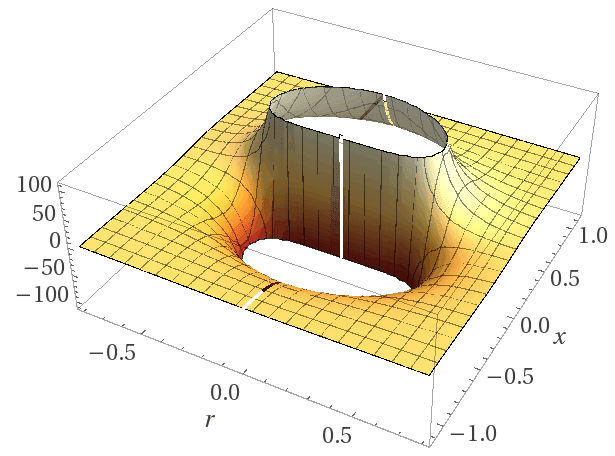
\includegraphics[width=0.8\textwidth]{Pictures/Figure_primitivePlot.png}}
  					\caption*{$\hat{\varphi}\in C^\infty (\mathbb{R}^{n+1}\setminus{0})$ \\ in cylindrical coordinates $(x=x^0,r)$}
					\end{figure}							
				\end{flushright}
				\vspace{-3.5ex}
			%
	 	 	\end{column}
 	 \end{columns}
	\end{propblock}
\end{frame}
%----------------------------------------------------------------------------------------------------------------------------------





%----------------------------------------------------------------------------------------------------------------------------------
\begin{frame}


		\begin{propblock}[The central pentagon commutes]
			\centering
			\parbox{0.96\linewidth}{%
				Consider ~$\alpha_i \in \Omega_{\text{Ham}}^{n-1}$,
				~$\gamma_i \in \bigoplus_{i=0}^{n-2}\Omega^n$,
				\\
				denote ~$e_i = \alpha_i + \gamma_i \in L(M,\omega)$, 
				~$v_i = v_{\alpha_i}$,  ~then:
			}
			\begin{columns}[T]
				\begin{column}{.8\linewidth}
					\begin{displaymath}
						\begin{split}
							\tilde{f}_k(e_1,\dots,e_k) =&~
							f_k(e_1,\dots,e_k)  + (-)^k \iota_{x_1}\dots\iota_{x_1} \chi
							\\
							(\tau_B)_k (e_1,\dots,e_k) =&~
							\begin{cases}
								e_1 - \iota_{v_1} \chi & k=1 \\
								0	& k \neq 1
							\end{cases}
							\\
							(\Psi)_k (e_1,\dots,e_k) =&~
							\begin{cases}
								e_1 + v_1 & k=1 \\
								\frac{B_k}{c_k} 
							\underbrace{\langle\cdot,\cdot\rangle_-\circ\dots\circ\langle\cdot,\cdot\rangle_-}_{k ~\text{times}}(e_1,\dots,e_k)	& k \neq 1
							\end{cases}
							\\
							\langle e_1,e_2 \rangle_- =&~
							\frac{1}{2}\big(\iota_{v_1}(\alpha_2+\gamma_2)
							- \iota_{v_2}(\alpha_1+\gamma_1)\big)							
						\end{split}
					\end{displaymath}
				\end{column}
				%
				\begin{column}{.2\linewidth}
					\vspace{5em}
					\small
					$B_k$ = Bernoulli numbers \\
					$c_k$ = numerical constant
				\end{column}			
			\end{columns}		
		\end{propblock}



\end{frame}
%----------------------------------------------------------------------------------------------------------------------------------









%----------------------------------------------------------------------------------------------------------------------------------
\end{document}
%----------------------------------------------------------------------------------------------------------------------------------




